% !TEX program = xelatex
\documentclass{matthijs}

% Style for first and last page
\usepackage{wallpaper}
\usepackage{color}
%\definecolor{arobsblue}{HTML}{0e2642}
%\definecolor{arobsblue}{HTML}{0f2c4c}
\definecolor{arobsblue}{HTML}{0e335c}

% Gantt chart for chapter Planning
\usepackage{pgfgantt}

\usepackage{csquotes}
\usepackage{biblatex}
\addbibresource{project.bib}

% Versioning
\usepackage[maxdepth=2]{gitinfo2}

%\usepackage{atbegshi}
%\AtBeginShipout{
%	\begin{tikzpicture}[remember picture,overlay]
%		\fill (current page.north west) node[below right,fill=arobsblue,draw=arobsblue,minimum width=\paperwidth,minimum height=2ex] (box) {};
%	\end{tikzpicture}
%}

\begin{document}

	% Set language to English
	\taal{en}

	% Cover page
	\begin{titelpagina}
		\color{white}

		\titel{\vspace{50pt}Plan of Action}{\emph{Project Lane Detection using FPGA's}}
		\author{
			\begin{tabular}{r l}
				\textbf{Author:} & Matthijs Bakker{\color{white}\footnote{\color{white}\textsuperscript{1} s1142121@student.windesheim.nl}} \\
				\textbf{Course:} & HBO-ICT ESA Full-Time \\
				\\
				\textbf{Company:} & AROBS Transilvania SA, Cluj-Napoca, Romania \\
				\textbf{Company Supervisor:} & Pangyu Jeong \\
				\textbf{Windesheim Supervisor:} & Willie Conen \\
				\\
				\textbf{Version:} & 1.2 \\
				\textbf{Commit:} & \gitAbbrevHash @master \\
			\end{tabular}
			\vspace{8ex}
		}

		\ThisULCornerWallPaper{1.001}{asset_bg_first_page.jpg}
		
	\end{titelpagina}

	\pagenumbering{arabic}
	\thispagestyle{empty}
	
	\begin{inhoudspagina}

	\end{inhoudspagina}

	\pagenumbering{arabic}

	\begin{hoofdstuk}{Preface}


		This document describes how I am going to work on this project.
		It describes all the factors which will have significant impact on the lifespan of this project, and proposes how I should handle these factors to make the project a success.
		For this project, the scope definition is very important, because the assignment can be made too complex and too big to complete in the assigned timeframe.
		In \verwijzing{paragraaf}{Scope} I will describe exactly what the project does and does not entail.
		
		\bigskip

		Not only is this document a guideline for myself; I hope that it also gives clarity to the project stakeholders.
		The stakeholders should be able to tell from this document how the project will be structured, which products will be created, when certain events will take place and what the potential pitfalls are.

		\bigskip

		Lastly, the planning of this project is described in \verwijzing{hoofdstuk}{Planning}.
		In the Gantt chart included with this document is visible how much time is allocated for each of the stages of this project.
		Important milestones, like the evaluations and presentations, are also visualized in this chart.
		
		\vspace{16pt}

		\begin{tabel}{Abbrevations}{l @{\extracolsep{\fill}} r}
			\textbf{Abbrevation} & \textbf{Explanation} \\
			\midrule
			FPGA & Field Programmable Gate Array; a customizable logic circuit \tabularnewline
			Xilinx Vivado & A design suite for developing digital logic solutions \tabularnewline
			SIP & Solo Iterative Process; an agile planning method \tabularnewline
			ADAS & Advanced Driver-Assistance System \tabularnewline
		\end{tabel}

	\end{hoofdstuk}
	
	\begin{hoofdstuk}{Project Definition}

		The goal of this project is to enable vehicles to be more autonomous by making them detect the road lane they're driving on.
		AROBS is continually improving vehicles by making them require less input from the driver while not compromising the safety of the vehicle.
		A system to detect if the vehicle is driving within the road lane is needed to guide the car on the road and to improve safety by preventing it from veering off the road.
		This system will be built in-house, because we can make it cheaper and more performant than existing products.
		Additionally, we can better regulate the quality of the product by building it ourselves, because we will be directly involved with creating it.
		Previous projects at AROBS regarding obstacle detection and number plate recognition have provided knowledge of the inner workings of these technologies.
		The final product -- a lane detection system -- is a digital logic layer which can be run on a Field Programmable Gate Array (hereafter referred to as a FPGA).
		The digital logic layer will be able to detect the position of the vehicle relative to the road lane by processing video input from a camera mounted on the dashboard of the vehicle.

		\begin{paragraaf}{Initial Situation}
			
			A vehicle with a camera on the dashboard is the starting position for this project.
			I need to develop a solution which can detect the position of the vehicle relative to the road lane by analyzing the camera feed.
			The final product will be implemented in a Hardware Description Language, so that it is possible to run it on an FPGA.
		
		\end{paragraaf}

		\begin{paragraaf}{Scope}

			The final product, as described above, takes input and output from other subsystems of a vehicle.
			It is assumed that these subsystems and the input and output streams to them already exist within the context of the vehicle.
			Therefore, these subsystems are not in the scope of this project.
			
			Outside of the scope of the project are:

			\begin{enumerate}
			
				\item Handling video input from a camera located on the dashboard of the vehicle
				\item Propagating the results from the lane detection system to other subsystems of the vehicle
				\item Integrating the system in a vehicle
				\item Controlling the vehicle
			
			\end{enumerate}

		\end{paragraaf}

		\begin{paragraaf}{Dependencies}

			For this project I am dependant on the availability of a capable FPGA to run the final product on.
			This FPGA needs a substantial amount of LUTs and a proficient clocking circuit, because the digital logic component will run in real-time.
			
			Hardware synthesis, the process of "assembling" a digital logic layer from hardware description files, requires a lot of computing resources because it is a NP-Hard \cite{chu2006rtl} problem.
			Every time I make a change to the hardware description, it needs to be re-synthesized and meet timing constraints.
			Therefore, I need a powerful computer which can quickly re-synthesize the digital logic.

			\begin{enumerate}

				\item The Digilent Arty A7 FPGA board will be used to run the final project on
				\item A powerful laptop provided by AROBS will be used to verify, synthesize and implement the digital logic layer
				\item Digital Logic design tools (Xilinx Vivado ML Edition and Vitis Model Composer) will need to be available on the laptop
		
			\end{enumerate}

		\end{paragraaf}

		\begin{paragraaf}{Preconditions}

			This project has its background in multiple areas: image analysis, hardware design and pattern recognition.
			Sufficient knowledge of these areas must be available for me to learn from and to help me with the realisation phase of the project.

			\begin{enumerate}

				\item Learning sources about hardware design, image analysis and pattern recognition are available at the company
				\item The company supervisor is knowledgable on these topics

			\end{enumerate}

		\end{paragraaf}

	\end{hoofdstuk}

	\begin{hoofdstuk}{Deliverables}

		For this project I will deliver three separate, testable, products.
		All of them are proof-of-concepts; they will not be brought on the market, however, they will deliver vital knowledge for AROBS which can be used to further develop their Advanced Driver-Assistance System (ADAS) warning system for autonomous vehicles.
		At the end of the project, the products each need to meet the Definition of Done in order for them to be regarded as a success.
		An additional three documents will be delivered which describe the functional and technical working of the products.
		The timeframe for each of these deliverables is included in \verwijzing{hoofdstuk}{Planning}.

		\begin{paragraaf}{Research Paper}
		
			The first product is a research paper in which I will set up a literature study.
			I will compare the results of the literature study and go in-depth on how each applicable algorithm works.
			Not only will I compare the effectiveness of each algorithm, I will also research how feasible it is to implement it in hardware.
			This paper will need to adhere to the Code of Conduct for Applied Research \cite{andriessen2010gedragscode}.
		
		\end{paragraaf}

		\begin{paragraaf}{Computer Program}
		
			The second product is a computer program which implements the lane detection algorithms as researched in the Research Paper.
			This computer program will be used as a reference point for implementing the algorithm in hardware.
			It needs to load an image and apply the algorithm on it to detect the position of the car relative to the road lane.
			This program can also be used to compare the expected result to the result of the hardware implementation.
		
		\end{paragraaf}

		\begin{paragraaf}{Hardware Implementation}
		
			The third and final product is a hardware implementation of the selected algorithm from the research paper.
			It will be written in a hardware description language and designed to work on a Xilinx Artix-7 FPGA.
			A video feed will be processed and results will be visible in real-time.
			With this product, a great amount of functional and technical documentation will be written, which will be useful for AROBS when integrating such a product in a vehicle.
		
		\end{paragraaf}

		\begin{paragraaf}{Functional Design}

			In this document, the requirements and acceptance criteria of the system will be examined.
			It will give a clear picture of what functionality will be included with the end product and what the product owner can expect to receive.
			Although the products will not directly be used by the end user, their interests will also be represented.

		\end{paragraaf}

		\begin{paragraaf}{Technical Design}

			The knowledge which will be gained from this project will be vital to AROBS with regards to further developing their Advanced Driver-Assistance System.
			It is important to capture this knowledge, so that it can be used later on.
			This document will describe the inner workings of both the computer program and the hardware implementation.
			The design choices and the reasoning behind them will also be explained in this document.

		\end{paragraaf}

		\begin{paragraaf}{Testplan}

			To verify the working of the program and the hardware, a  
		\end{paragraaf}
	
	\end{hoofdstuk}

	\begin{hoofdstuk}{Approach}

		\begin{paragraaf}{Complexity Management}
			
			Because the final product is complex and vague in nature, I have divided the project into several concrete goals, each of which will give further clarification to what needs to be done for the final product.
			I can use these goals as stepping stones to work my way to implementing the algorithm on a FPGA.
			For example, it will be much more doable for me to implement the algorithm in hardware if I first implement it in a computer program that can run on the laptop.
			This program will also be used as a reference point to test if the algorithm works correctly in hardware, because the resulting images from the code -- which will be assumed to be the correct implementation -- can be compared to those that will be generated by the hardware.
		
		\end{paragraaf}

		\begin{paragraaf}{Agile Techniques}
			
			At Windesheim we have always used the Scrum technique to work on projects.
			However, this technique can\'t be used when working on a project alone: the goal of scrum is to have multiple people governing different tasks and representing stakeholders \cite{gant2019scrum}.
			Therefore, I will be using the Solo Iterative Process \cite{dorman2012sip} (later referred to as \textit{SIP}) technique.
			Using this technique, I can manage an iterative feedback loop, similar to what you would do with Scrum sprints.
			I can integrate feedback from the stakeholders and analyze the impact of my actions in each iteration of this loop.
			During each iteration, I will pick up a task and make a Minimum Viable Product (MVP) that meets the Definition of Done.
			Between iterations, I will reflect on the progress of the project.

			\begin{figuur}{A visualization of the SIP-technique}

				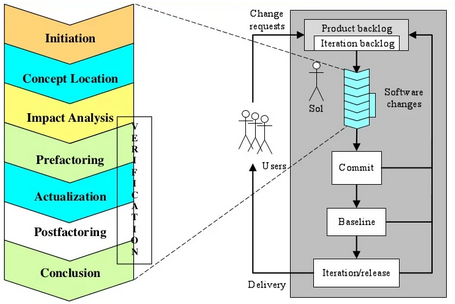
\includegraphics[width=0.5\textwidth]{sip.png}  \cite{dorman2012sip}

			\end{figuur}

			It is one of my personal goals to improve the way I work on projects alone, because I usually procrastinate too much or add too much unwanted functionaity to something just because I feel like it.
			By using this technique for the first time, I want to try it out and bring some of the habits of this technique to my own planning.
		
		\end{paragraaf}

		\begin{paragraaf}{Version Management}

			The code and documentation will be stored in a Git repository.
			Because every change to these files is recorded in the commit log, the files can be restored to a point back in time, if required.
			It can also be viewed which change was made at which time.
			The repository will be hosted on GitHub so that the code safely stored and available at any time.
			All commits will be signed using PGP so that the validity of them can be cryptographically confirmed.
			
			\bigskip
			
			The documentation will be written in LaTeX, except for some documents which are required to be submitted in \textit{docx} format, as described in the Internship and Graduation Manual \cite{windesheim2021handleiding}.
			The reason behind this choice is because LaTeX is a flexible language written in plaintext files.
			Last project, our working group encountered many issues with Microsoft Word, with large documents frequently corrupting or the program crashing.
			Another justification for using LaTeX is that the bibliography is easily integrated with the document.
			These documents can be exported to PDF/A, as required by the Internship and Graduation Manual \cite{windesheim2021handleiding}.

		\end{paragraaf}

		\begin{paragraaf}{Sequence}

			As described in \verwijzing{hoofdstuk}{Planning}, I will start this project with the research paper.
			This is the first deliverable, and it will help me with choosing the most approriate algorithm for use in the second deliverable.
			After the research has been completed, I will realise a computer program, as described in \verwijzing{paragraaf}{Computer Program}.
			Finally, as mentioned in \verwijzing{paragraaf}{Hardware Implementation}, the proof-of-concept hardware description will be made.
			It will be made suitable to run on the FPGA board.
			
		\end{paragraaf}

	\end{hoofdstuk}

	\begin{hoofdstuk}{Organization}

		\begin{paragraaf}{The Company}

			AROBS is a multinational company focused on software engineering. It's main focus is on the Automotive Sector, having developed internationally used products such as a vehicle tracking system and on-board computers.
			At the Automotive Department, where I will be stationed during the internship, work more than 400 of its employees.
			The main office is located in the Cluj Business Center in Cluj-Napoca, Romania.
			Internally, Skype and Microsoft Teams are used for quick and direct communication.

		\end{paragraaf}

		\begin{paragraaf}{Stakeholders}

			\bigskip
			
			\begin{tabular*}{\textwidth}{l @{\extracolsep{\fill}} r}
				\toprule
				Name & Matthijs Bakker \tabularnewline
				Role & Intern, Student HBO-ICT ESA \tabularnewline
				E-mail & s1142121@student.windesheim.nl \tabularnewline
				E-mail & matthijs.bakker@arobs.com \tabularnewline
				Phone & +31 6 47122597 \tabularnewline
				PGP & B052 6642 ACBE 5FB0 \tabularnewline
				\bottomrule
			\end{tabular*}
			
			\vspace{4ex}

			\begin{tabular*}{\textwidth}{l @{\extracolsep{\fill}} r}
				\toprule
				Name & Pangyu Jeong \tabularnewline
				Role & Company Supervisor \tabularnewline
				E-mail & pangyu.jeong@arobs.com \tabularnewline
				\bottomrule
			\end{tabular*}

			\vspace{4ex}

			\begin{tabular*}{\textwidth}{l @{\extracolsep{\fill}} r}
				\toprule
				Name & Willie Conen \tabularnewline
				Role & Windesheim Supervisor \tabularnewline
				E-mail & w.h.conen@windesheim.nl \tabularnewline
				\bottomrule
			\end{tabular*}

			\vspace{4ex}

			\begin{tabular*}{\textwidth}{l @{\extracolsep{\fill}} r}
				\toprule
				Name & Windesheim HBO-ICT \tabularnewline
				Role & Training Institute \tabularnewline
				E-mail & ictstageafstuderen@windesheim.nl \tabularnewline
				\bottomrule
			\end{tabular*}

		\end{paragraaf}

	\end{hoofdstuk}

	\begin{hoofdstuk}{Management Strategies}

		\begin{paragraaf}{Risk Management}

			There exist a few scenarios which could hinder the progress of the project.
			For each scenario, I have approximated the impact it would have on the project and the chance of it happening.
			These can be found in the enumeration below.

			\begin{enumerate}

				\item	Lack of hardware availability -- impact: low, chance: low --
					It may happen that the FPGA board or other hardware required in this project gets broken or is unavailable when needed.
					Fortunately, AROBS can buy replacement hardware within 1-3 days of notice.
				
				\item	Lack of time -- impact: medium, chance: low --
					When improperly planned, projects can run out of time.
					For this reason, I chose to incorporate SIP, a standardised approach to planning, into this project.
					If this does occur, it will be mentioned in progress reports and I will fall back to a \enquote{KISS-approach}.

				\item	Office closure due to the Coronavirus -- impact: high, chance: medium --
					If COVID-19 gets out of hand, the Romanian government may decide to issue a lock-down in parts of the country.
					I have received a work laptop from AROBS which I may carry back to my apartment to work from home.
					I won't be able to take the rest of the hardware back home, which is why the project may be hindered.

			\end{enumerate}

		\end{paragraaf}
		
		\begin{paragraaf}{Quality Management}

			The quality of the products will be assured by having them adhere to well-known guidelines.
			The research paper needs be written in accordance to the Code of Conduct for Applied Research \cite{andriessen2010gedragscode} and needs to have a substantiated explanation.
			The result of the research paper is important, because it will have a big impact on the course of this project, which is why it needs to be re-evaluated and to be reflected upon.
			
			\bigskip

			In the technical documentation, multiple layers of abstraction will be used, similar to the C4 model \cite{brown2018the}.
			This helps to create a bigger picture of how parts of the system communicate with each other.
			It also makes the system understandable for non-technical people by separating the underlying ideas from the specific implementation details.

			\bigskip

			A Definition of Done will make sure that a part of the system is up-to-standard before being marked as \enquote{done}. It reads as follows:
			
			\begin{enumerate}
				\item The code has been formally verified and tested
				\item The code has been provided with comments
				\item The code has been integrated into the codebase
				\item The code has been merged into the primary branch of the repository
				\item The technical documentation has been updated, reflecting the current state of the product
				\item The SIP-documents have been updated to reflect the state of the current iteration
			\end{enumerate}

		\end{paragraaf}

		\begin{paragraaf}{Configuration Management}

			As described in \verwijzing{paragraaf}{Version Management}, all documentation and code regarding this project will be managed in a Git repository.
			This allows me to track changes over time and gives me the opportunity to revert to a previous version, if needed.
			As noted in \verwijzing{hoofdstuk}{Planning}, the final portfolio needs to be handed in Week 18.
			I will compile all project documents to PDF/A and submit them to the Windesheim ELO in this week.
			
		\end{paragraaf}

		\begin{paragraaf}{Communication Strategy}

			For communication between colleagues at AROBS, Skype will be used, because it is the de-facto way of communication at the company.
			Between the company and Windesheim, all communication will be exchanged via e-mail.
			
			\bigskip
			
			On a weekly basis, I will make a progress report, which will first be amended upon and approved by the Company Supervisor before being sent via e-mail to the Windesheim Supervisor.
			If required, a stakeholder may request communication via PGP-signed messages to ensure the validity of them.

		\end{paragraaf}

	\end{hoofdstuk}

	\begin{hoofdstuk}{Personal Development}

		I have set two learning goals for myself as part of this project:

		\begin{enumerate}
			\item Learn how to efficiently plan projects and divide a complex project into smaller steps with the Solo Iterative Process technique. I usually procrastinate too much, thinking about how I can make something better without actually improving it. I want to learn how to use this planning method and incorporate parts of it into my personal planning. By using this technique in the project, I will be familiarizing myself with it, and teaching myself the important aspects of planning.
			\item Immerse myself in the world of image analysis by getting hands-on experience. I've always been fascinated with how computers -- simple electronic circuits with electricity running through them -- can do human-like pattern recognition. I want to grasp the concept behind image analysis and improve my knowledge on it. AROBS offers me digital learning materials such as instructional videos and courses on this subject.
		\end{enumerate}

		Aside from these goals, I will also learn what it's like to work abroad and how different cultures and ethnicities are integrated into a work environment.

	\end{hoofdstuk}

	\begin{hoofdstuk}{Planning}

		The project will be spread over a total of 21 weeks.
		The first week will start on \textit{Monday, 31 January 2022}.
		An approximate planning on a weekly basis can be viewed in \verwijzing{figuur}{Project Timeline visualized in a Gantt Chart}.
		Halfway the project, after the first term of 10 weeks, the first evaluation will take place.
		At the end of the project, the final assessment will take place and I will present the product to the company.
		The portfolio will be handed in on \textit{Thursday, 2 June 2022}.

		\begin{figuur}{Project Timeline visualized in a Gantt Chart}
			\begin{ganttchart}{1}{21}
				\gantttitle{Week \#}{21} \\
				\gantttitlelist{1,...,21}{1} \\

				\ganttgroup{Documentation}{1}{8} \\
				\ganttbar{Plan of Action}{1}{2} \\
				\ganttlinkedbar{Kick-Off}{2}{2} \ganttnewline
				\ganttlinkedbar{Research Paper}{3}{7} \ganttnewline
				\ganttbar[bar left shift=0.5]{Algorithm Implementation}{4}{8} \ganttnewline
				\ganttmilestone{Mid-Term Evaluation}{8} \ganttnewline
				\ganttgroup{Realisation}{9}{16} \ganttnewline
				\ganttbar{Design}{9}{10} \ganttnewline
				\ganttbar{FPGA Implementation}{11}{16} \ganttnewline
				\ganttmilestone{Presentation}{10} \ganttnewline
				
				\ganttgroup{Evaluation}{17}{21} \ganttnewline
				\ganttbar{Portfolio}{17}{18} \ganttnewline
				\ganttmilestone{Final Evaluation}{17} \ganttnewline
				\ganttmilestone{Portfolio Hand-in}{18} \ganttnewline
				\ganttbar{Presentations}{20}{21} \ganttnewline
				
				\ganttlink{elem4}{elem7}
				\ganttlink{elem7}{elem8}
				\ganttlink{elem8}{elem11}
				\ganttlink{elem11}{elem14}

			\end{ganttchart}
		\end{figuur}
		
	\end{hoofdstuk}

	% Bibliography page
	\begin{hoofdstuk}{References}
		\printbibliography[heading=none]
	\end{hoofdstuk}

	% Empty last page
	\clearpage
	\thispagestyle{empty}
	\addtocounter{page}{-1}
	\ThisULCornerWallPaper{1.005}{asset_bg_last_page.jpg}
	\
	\clearpage

\end{document}
